\documentclass[tikz,border=0cm,dvipsnames,x11names,rgb]{standalone}

\usepackage{amsmath,amssymb,amsfonts}
\usetikzlibrary{calc,
fit,
shapes.misc,
shapes.geometric,
arrows.meta,
fadings,
matrix,
chains,
scopes,
positioning}

\usepackage{pgfplots}
\usepackage{pgfplotstable}
\pgfplotsset{compat=1.18}



\usepackage[]{fontspec}

\setmainfont{Latin Modern Roman}
\setmonofont{Latin Modern Math}
\renewcommand{\textsc}[1]{{\fontfamily{lmr}\selectfont \scshape #1}}

\usepackage[]{bm}

\makeatletter
\@ifundefined{fromRoot}{\newcommand{\fromRoot}[1]{../../#1}}{}

\def\input@path{{../..}{..}{.}{./svg}{./pgfplots}{./tikzpicture}}
%or: \def\input@path{{/path/to/folder/}{/path/to/other/folder/}}
\makeatother

\newcommand*{\gf}[1]{\acrshort{gf}($#1$)}%
\newcommand*{\mpn}[1]{\bm{P}_{#1}}%
\newcommand*{\pn}[1]{%
  \ifthenelse{\equal{#1}{}}{$\mpn{0}$}{$\mpn{#1}$}%
}%

\newcommand*{\pk}[3]{%
  \ifthenelse{\equal{#1}{#2}}{\textcolor{red}{\phantom{.}$p_0$\phantom{.}}}{\phantom{.}$p_#3$\phantom{.}}%
}%


\newcommand*{\placeholder}{
\includegraphics[width=\linewidth, height=.25\textheight, keepaspectratio = true]{figures/certified_xilinx.png}}%

\newcommand*{\snr}{\acrshort{snr}}%
\newcommand*{\snrs}{\acrshortpl{snr}}%

\newcommand*{\mpd}[0]{p_\Delta}%
\newcommand*{\mpo}[0]{p_\omega}%
\newcommand*{\pd}[0]{$\mpd$}%
\newcommand*{\po}[0]{$\mpo$}%
\newcommand*{\mpfa}[0]{\mathcal{P}_{fa}}%
\newcommand*{\mpmd}[0]{\mathcal{P}_{md}}%
\newcommand*{\pfa}[0]{\acrshort{pfa}}%
\newcommand*{\pmd}[0]{\acrshort{pmd}}%
\newcommand*{\mnorm}[1]{\mathcal{L}_{#1}}%
\newcommand*{\norm}[1]{$\mnorm{#1}$}%
\newcommand*{\fft}{\acrshort{fft}}%
\newcommand*{\mfft}[1]{\mathcal{F}(#1)}%
\newcommand*{\mifft}[1]{\mathcal{F}^{-1}(#1)}%
\newcommand*{\ts}{\acrshort{ts}}%

\newcommand*{\cpp}[1]{C\textrm{++#1}}%
\newcommand*{\na}{\textrm{\textcolor{SlateGray4}{N/A}}}%

\newcommand*{\vect}[1]{\bm{#1}}%
\newcommand*{\mat}[1]{\bm{\mathrm{#1}}}%

\newcommand*{\task}[1]{\mathcal{T}_{#1}}%

\newcommand*{\sdr}{\acrshort{sdr}}%
\newcommand*{\fpga}{\acrshort{fpga}}%



\begin{document}

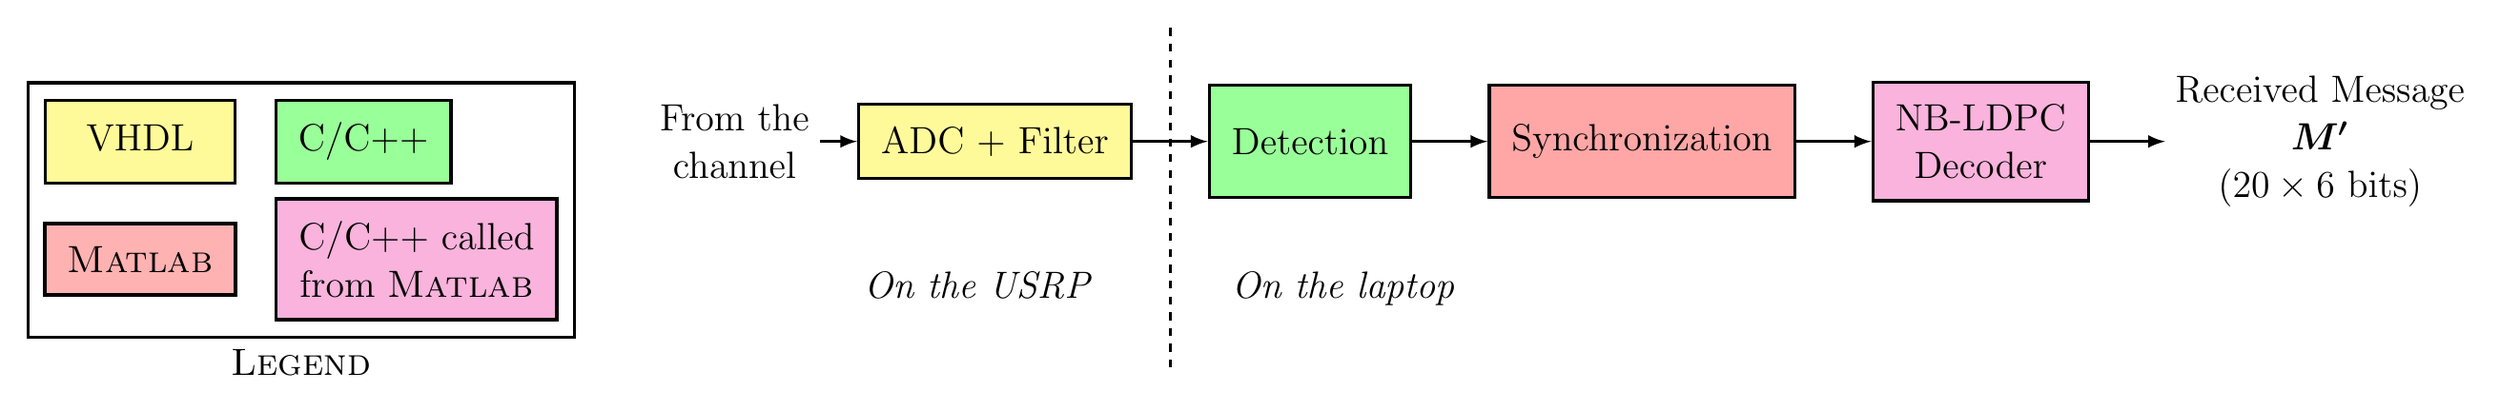
\begin{tikzpicture} [-latex,
    >=latex,
    auto,
    very thick,
    main node/.style={rectangle, fill = white!35, draw,
        align=center, inner sep = 3 mm},
    every node/.style={font=\Large}
  ]

  \node [
    align=center,
    minimum height = 1.5cm
  ] (chan) at (0, 0) {From the\\
  channel};

  \node [main node,
  align=center,
  minimum height = .75cm,
  minimum width = .5cm,
  fill = yellow!40,
  % label = above:{$f_s = 500$ kHz},
  right = .5cm of chan
  ] (adc) {ADC $+$ Filter};

  \draw (chan.east) -- (adc.west);
  \draw [dashed, -] ($(adc.north east) + (.5, 1)$) -- ($(adc.south east) + (.5, -2.5)$);
  
  \node [anchor = south east, inner sep = .8cm] at ($(adc.south east) + (.5, -2.5)$) {\itshape On the USRP\phantom{p}};
  \node [anchor = south west, inner sep = .8cm] at ($(adc.south east) + (.5, -2.5)$) {\itshape On the laptop};

  \node [main node,
    minimum height = 1.5cm,
    fill = green!40,
    %minimum width = 3cm,
    right = 1 cm of adc
  ] (ccskd)  {Detection};


  \draw (adc.east) -- (ccskd.west);

  \node [main node,
    fill = red!35,
    minimum height = 1.5cm,
    %minimum width = 3cm,
    right = 1 cm of ccskd
  ] (ccsks) {Synchronization};

  \draw (ccskd.east) -> (ccsks.west);

  \node [main node,
    fill = magenta!30,
    minimum height = 1.5cm,
    right = 1cm of ccsks
  ] (nbdec) {NB-LDPC\\Decoder};

  \node [right = 1cm of nbdec, align=center] (Mp) {Received Message\\$\vect{M'}$\\($20 \times 6$ bits)};


  \draw (ccsks.east) -> (nbdec.west);


  \draw (nbdec.east) -> ($(1, 0) + (nbdec.east)$);


  %\draw ($(-1, 0) + (ccskd_z.west)$) -> (ccskd_z.west);

  %\draw (ccsks.east) -> ($(1, 0) + (ccsks.east)$);

  %\draw [dashed, color = red!50!gray, -] (anchor.south west) -- (frame_chosen.north west);
  %\draw [dashed, color = red!50!gray, -] (anchor.south east) -- (frame_chosen.north east);

  \node [
    main node,
    draw,
    left = 5.5 cm of chan,
    fill=yellow!40,
  ] (rcvl) {\phantom{/}VHDL\phantom{/}};
  \node [
    main node,
    draw,
    right = .5cm of rcvl,
    fill=green!40,
  ] (rccc) {C/\cpp{}};
  \node [
    main node,
    draw,
    below = .5cm of rcvl,
    fill=red!30,
  ] (rcm) {\textsc{Matlab}};
  \node [
    draw,
    main node,
    align = center,
    right = .5cm of rcm,
    fill=magenta!30,
  ] (rcmc) {C/\cpp{} called\\from \textsc{Matlab}};

  \node[
    draw,
    inner sep = 2.1 mm,
    fit = (rcvl) (rcmc),
    label = {below:\textsc{Legend}}
  ] (rcfit) {};

\end{tikzpicture}

\end{document}
